\documentclass{llncs}
\usepackage{amsmath}
\usepackage{mathtools,amssymb}
\usepackage{xcolor}
\usepackage[
bookmarks=false,
breaklinks=true,
colorlinks=true,
linkcolor=black,
citecolor=black,
urlcolor=black,
%pdfstartpage=19,
pdfpagelayout=SinglePage,
pdfstartview=Fit
]{hyperref}
\usepackage{tikz}
\usepackage{pgf}
\usetikzlibrary{fit,matrix,arrows,petri,topaths,positioning,automata,shapes,calc,backgrounds,chains,scopes,graphs}
\tikzset{circle split part fill/.style  args={#1,#2}{%
 alias=tmp@name, 
  postaction={%
    insert path={
     \pgfextra{% 
     \pgfpointdiff{\pgfpointanchor{\pgf@node@name}{center}}%
                  {\pgfpointanchor{\pgf@node@name}{east}}%            
     \pgfmathsetmacro\insiderad{\pgf@x}
      \fill[#1] (\pgf@node@name.base) ([xshift=-\pgflinewidth]\pgf@node@name.east) arc
                          (0:180:\insiderad-\pgflinewidth)--cycle;
      \fill[#2] (\pgf@node@name.base) ([xshift=\pgflinewidth]\pgf@node@name.west)  arc
                           (180:360:\insiderad-\pgflinewidth)--cycle;            
         }}}}}

\begin{document}

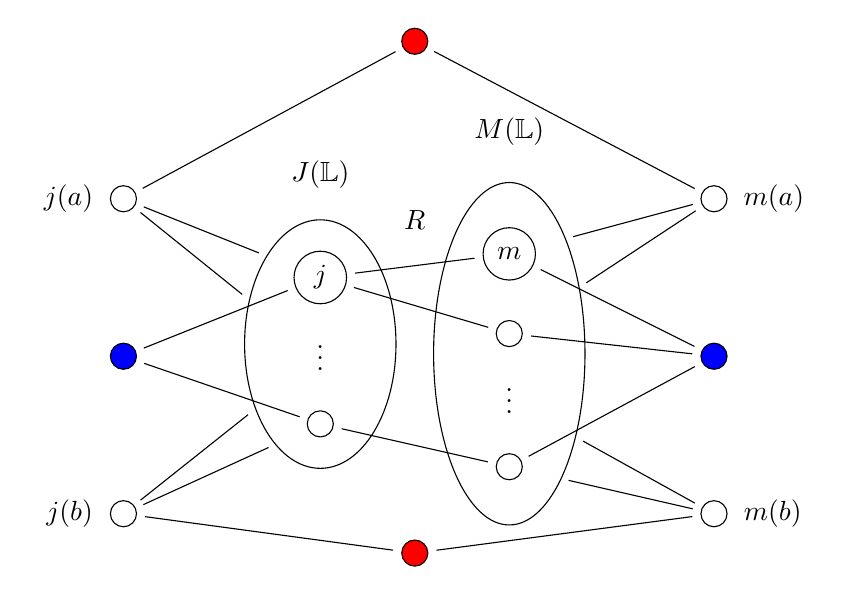
\begin{tikzpicture}[every node/.style={draw,circle},fsnode/.style={fill=white},ssnode/.style={fill=white},bbnode/.style={fill=blue},rrnode/.style={fill=red},
				every fit/.style={ellipse,draw,inner sep=-2pt,text width=1.5cm},shorten >= 3pt,shorten <= 3pt,scale=0.6]				
				% the vertices of U
				\begin{scope}[start chain=going below,node distance=5mm]
					\node[fsnode,on chain] (f1){$j$};
					\node[white,on chain,label={[xshift=0cm, yshift=-0.5cm]$\vdots$}] (f2){};
					\node[fsnode,on chain] (f3){};
				\end{scope}				
				% the vertices of V
				\begin{scope}[xshift=4cm,yshift=0.5cm,start chain=going below,node distance=5mm]
					\node[ssnode,on chain] (s4){$m$};
					\node[ssnode,on chain] (s5){};
					\node[white,on chain,label={[xshift=0cm, yshift=-0.5cm]$\vdots$}] (s6){};
					\node[ssnode,on chain] (s7){};					
				\end{scope}				
				
				\node [black,fit=(f1) (f3),label=above:$J(\mathbb{L})$] {};				
				\node [black,fit=(s4) (s7),label=above:$M(\mathbb{L})$] {};							
				\node [white,yshift=0.2cm,xshift=1.2cm,label=above:{$R$}] {};
				\node[bbnode,yshift=-1cm,xshift=5cm] (s8){};
				\node[bbnode,yshift=-1cm,xshift=-2.5cm] (f4){};
				
				\node[fsnode,yshift=1cm,xshift=5cm,label=right:$m(a)$] (s9){};
				\node[fsnode,yshift=1cm,xshift=-2.5cm,label=left:$j(a)$] (f5){};
				
				\node[fsnode,yshift=-3cm,xshift=5cm,label=right:$m(b)$] (s10){};
				\node[fsnode,yshift=-3cm,xshift=-2.5cm,label=left:$j(b)$] (f6){};
				
				\node [rrnode,yshift=3cm,xshift=1.2cm] (x){};
				\node [rrnode,yshift=-3.5cm,xshift=1.2cm](y){};
				
				\draw[shorten >=0.5cm] (f5) -- (f1);
				\draw[shorten >=1.1cm] (f5) -- (f2);
				\draw[shorten >=1cm] (f6) -- (f2);
				\draw[shorten >=0.55cm] (f6) -- (f3);
				
				\draw[shorten >=0.5cm] (s9) -- (s4);
				\draw[shorten >=1cm] (s9) -- (s5);
				\draw[shorten >=0.9cm] (s10) -- (s6);
				\draw[shorten >=0.6cm] (s10) -- (s7);
				
				\draw (x) -- (s9);
				\draw (x) -- (f5);
				\draw (y) -- (s10);
				\draw (y) -- (f6);
				
				% the edges
				\draw (f4) -- (f1);
				\draw (f4) -- (f3);				
				\draw (s8) -- (s4);
				\draw (s8) -- (s5);
				\draw (s8) -- (s7);
				
				\draw (f1) -- (s5);
				\draw (f1) -- (s4);				
				\draw (s7) -- (f3);
			\end{tikzpicture}

\end{document}